\documentclass{article}

\usepackage[a4paper, total={7in, 10in}]{geometry}
\usepackage{times}
\usepackage{graphicx}
\usepackage{amsmath}
\usepackage{enumitem}
\usepackage{titlesec}
\usepackage{fancyhdr}
\usepackage{hyperref}
\usepackage{caption}
\usepackage{float}
\usepackage{cite}
\usepackage[vietnamese]{babel}

% ==== IEEE-style Custom Formatting ====
\renewcommand{\thesection}{\Roman{section}} % Số La Mã cho Section


\titleformat{\section}
  {\normalfont\bfseries\uppercase}{\thesection.}{1em}{}
\titleformat{\subsection}
  {\normalfont\itshape}{\thesubsection}{1em}{}

\setlength{\parskip}{0pt}
\setlength{\parindent}{1em}
\linespread{1.0}
\setlength{\columnsep}{0.25in}
% =====================================

\pagestyle{fancy}
\fancyhf{}
\rhead{ICT Research and Applications}
\lhead{Vol. 2025, No. 1, April}
\cfoot{\thepage}

\title{\textbf{\LARGE BUILDING A DEEP LEARNING-BASED TEXT SUMMARIZATION MODEL}}
\author{
Hoang Bao Viet, 
Nguyen Huyen Trang, 
Nguyen Thi Ha Phuong \\
The University of Danang, Vietnam - Korea University of Information and Communication Technology
}

\date{}

\begin{document}
\sloppy

\twocolumn[
\maketitle
\vspace{-2em}

\vspace{1em}
\section*{Abstract}
\addcontentsline{toc}{section}{Abstract}
Automatic text summarization is an important task in Natural Language Processing (NLP). This paper proposes a deep learning-based text summarization model for Vietnamese using the Transformer architecture. The model is trained on Vietnamese news datasets and evaluated using the ROUGE metric. Experimental results demonstrate that the proposed approach outperforms traditional summarization methods.

\textbf{Keywords:} text summarization, deep learning, Transformer, NLP, Vietnamese
\vspace{1em}
]

\section{Introduction}

\subsection{Motivation}
In the era of digital commerce, user-generated reviews on social media and e-commerce platforms have emerged as an essential source of consumer insight and product feedback. These reviews influence purchasing decisions, brand perception, and product development across various industries. However, the vast volume, variability, and often redundant nature of such content pose a significant challenge for both end-users and businesses attempting to extract actionable information. Automatic text summarization, particularly through deep learning (DL)-based approaches, has been increasingly adopted to generate concise and informative summaries of user reviews.

Despite substantial advances in automatic summarization in resource-rich languages such as English, Chinese, and Japanese, supported by large benchmark datasets and robust pretrained language models, progress in Vietnamese remains modest. Vietnamese reviews—especially those related to smartphones on local e-commerce platforms—are typically short, highly unstructured, and infused with informal expressions, abbreviations, and domain-specific slang. These linguistic and contextual peculiarities present significant challenges that impede the direct application of existing summarization techniques.
\subsection{Scope of the Survey}
This survey investigates deep learning-based approaches for summarizing Vietnamese product reviews, with a specific focus on reviews collected from social media and e-commerce platforms. We concentrate on methods that generate summaries which are both concise and comprehensive, minimizing redundancy while capturing essential and sometimes infrequent insights. The paper emphasizes approaches applicable to low-resource and noisy settings, as exemplified by Vietnamese language data.

We further analyze the suitability of modern architectures, such as transformer-based models, transfer learning strategies, and hybrid methods, in handling the unique demands of Vietnamese user-generated text. In addition, this survey introduces a practical case study using a self-constructed dataset of smartphone reviews, which demonstrates the real-world limitations of existing models and the critical need for more tailored solutions.

\subsection{Contributions}
This survey contributes to the advancement of automatic text summarization in low-resource languages by offering a comprehensive examination of deep learning-based methods, encompassing both extractive and abstractive paradigms. It places particular emphasis on the Vietnamese context, where user-generated product reviews present unique challenges due to informal language usage, syntactic irregularities, and the scarcity of annotated training resources.

Through a critical evaluation of state-of-the-art techniques, including transformer-based architectures, prompt-driven approaches, and hybrid models, the paper explores their adaptability and performance limitations when applied to Vietnamese-language data. In doing so, it reveals a substantial gap between the capabilities of current multilingual summarization systems and the specific demands posed by low-resource, domain-focused settings.

Moreover, the survey identifies several key directions for future research, highlighting the importance of data-centric methodologies, context-sensitive evaluation metrics, and models designed to accommodate the linguistic nuances of Vietnamese. Collectively, these insights aim to guide the development of more robust, scalable, and linguistically aware summarization systems for Vietnamese and other under-resourced languages.

\vspace{1em}
\section{Background and Terminologies}
Automatic text summarization is the process of generating a concise and coherent version of a longer text while preserving its key information. It is broadly categorized into two major types: \textit{extractive summarization} and \textit{abstractive summarization}. Extractive methods identify and select salient phrases or sentences directly from the source text, often ranking them based on statistical or learned importance. These approaches are generally easier to implement and less prone to factual errors, but they may produce summaries that are disjointed or lack coherence. In contrast, abstractive methods generate novel sentences that may paraphrase or rephrase the original content, closely mimicking how a human might summarize. While this allows for more fluent and compact summaries, it requires deeper semantic understanding and poses greater modeling challenges, particularly in low-resource languages.

In addition to this core distinction, summarization tasks can be classified as \textit{single-document} or \textit{multi-document}. The former involves condensing information from a single text source, such as a user review or a product description, whereas the latter synthesizes information from multiple related sources. In the context of e-commerce and social media, multi-document summarization is especially relevant, as product reviews often appear in clusters under a single listing and need to be summarized collectively to reflect diverse user perspectives.

The advent of deep learning has significantly advanced the capabilities of summarization systems. Early deep learning models relied on recurrent neural networks (RNNs) and their gated variants—LSTM and GRU—to encode input sequences and generate summaries in a sequential manner. These sequence-to-sequence (seq2seq) models provided a data-driven alternative to rule-based or statistical summarization. However, they often struggled with long-range dependencies and information retention, especially in multilingual settings.

To address these limitations, attention mechanisms were introduced, allowing the model to selectively focus on different parts of the input during generation. This innovation led to the development of transformer-based architectures, which entirely replaced recurrence with self-attention mechanisms. Models such as BERT, GPT, T5, and BART have since defined the state-of-the-art in both extractive and abstractive summarization. These models leverage massive pretraining on general corpora and can be fine-tuned on specific tasks or adapted via prompting strategies.

While such architectures have yielded impressive results in English and other high-resource languages, their application to Vietnamese remains underexplored. The absence of large-scale annotated summarization datasets in Vietnamese and the presence of informal, fragmented user-generated content complicate both model training and evaluation. As we explore in subsequent sections, adapting these foundational models to the Vietnamese context requires addressing linguistic nuances and data constraints that are often absent in mainstream research.

\vspace{1em}
\section{Related Works}

\subsection{Global Research Landscape in Summarization}

The field of automatic text summarization has witnessed rapid advancements over the past decade, largely driven by the availability of large-scale datasets and powerful pretrained models in high-resource languages. Several publicly available corpora have become standard benchmarks for evaluating summarization models. For instance, the CNN/DailyMail dataset contains long-form news articles paired with multi-sentence summaries, enabling both extractive and abstractive modeling. The XSum dataset presents a more challenging setting, requiring models to produce highly concise, one-sentence summaries. Other corpora such as Gigaword, Reddit TIFU, and Multi-News contribute to modeling diversity by including informal, user-generated, or multi-document input. These datasets share a common advantage: they are well-formatted, consistently structured, and linguistically clean—conditions rarely met in low-resource languages such as Vietnamese.

\subsection{Evaluation Metrics}

To evaluate performance on these datasets, most studies rely on automatic metrics, particularly the ROUGE family, which measures n-gram overlap between system outputs and reference summaries. ROUGE-1 and ROUGE-2 assess unigram and bigram precision and recall, while ROUGE-L captures longest common subsequences. BLEU, originally proposed for machine translation, is occasionally used, although it is less sensitive to paraphrased content. More recently, semantic similarity metrics such as METEOR and BERTScore have gained traction, as they better capture meaning beyond surface-level overlap. Nevertheless, all these metrics face limitations when applied to subjective, informal, and opinion-rich texts like product reviews. They are also language-dependent, and their reliability may degrade in Vietnamese due to tokenization inconsistencies and sparse lexical overlap between human and machine summaries.

\subsection{Methodological Trends}

From a methodological perspective, the landscape has evolved significantly with the rise of deep learning. Early work in summarization applied sequence-to-sequence (seq2seq) models with attention mechanisms, but more recent approaches leverage transformer-based models pretrained on massive corpora. Models such as BART and T5 are now commonly fine-tuned for summarization tasks, achieving state-of-the-art results in many benchmarks. In multilingual contexts, models like mBART and mT5 have been proposed, offering cross-lingual capabilities that potentially benefit low-resource languages through parameter sharing and transfer learning.

\subsection{Prompt-based and Multi-task Learning}

In parallel, prompt-based learning has emerged as a lightweight yet powerful alternative to fine-tuning. Instead of modifying model weights, these methods frame tasks as natural language prompts fed into a pretrained model, such as GPT-3 or T0. This strategy reduces the dependence on labeled data and has been shown to perform competitively on summarization benchmarks. Additionally, multi-task learning has gained attention for its ability to share representations across related tasks—such as sentiment classification and summarization—particularly useful in domains like product reviews where sentiment is often entangled with summary-worthy content.

\subsection{Limitations and Transferability}

Despite these advances, the overwhelming majority of studies and datasets remain concentrated in English and a handful of other well-resourced languages. Consequently, the generalizability of these models to Vietnamese, especially in domains characterized by informal, user-generated text, remains an open question. The next section will examine these challenges in greater detail, providing a Vietnamese-centric view on the limitations of existing tools and highlighting opportunities for future work.
\section{The Vietnamese Context}

\subsection{Linguistic Challenges}

Vietnamese presents several unique linguistic features that complicate the task of text summarization. Unlike many Indo-European languages, Vietnamese is an analytic language, meaning it relies heavily on word order rather than inflections for grammatical structure. Additionally, Vietnamese is known for its tonal nature, where the meaning of a word can change based on its tone. These characteristics, while enriching in everyday communication, pose challenges for natural language processing (NLP) tasks, as they require models to carefully account for context and meaning without relying on traditional syntactic cues.

Moreover, Vietnamese is marked by frequent use of informal expressions, including slang and abbreviations, which are especially prevalent in user-generated content like product reviews. Many users on e-commerce platforms utilize colloquial phrases and creative abbreviations (e.g., "pin trâu" for "long-lasting battery"), which may not be captured by conventional models trained on formal language. Furthermore, sentence structure in Vietnamese is often non-standard, with many sentences lacking clear subjects or objects, as well as ellipses that omit important syntactical elements. These factors significantly hinder the ability of standard summarization models to parse the text effectively, leading to difficulties in generating coherent and meaningful summaries.

\subsection{Dataset Constraints}

The availability of high-quality, annotated datasets is a critical factor in training deep learning models for text summarization. While large-scale datasets like CNN/DailyMail or XSum are readily available for languages such as English, Vietnamese datasets for summarization remain scarce. Most of the available data is either manually collected or limited to specific domains, often requiring significant preprocessing to handle informal language and ensure consistency in annotation.

Another challenge lies in the diversity of topics found in Vietnamese reviews. In the case of product reviews, for example, users discuss a wide range of features—such as performance, battery life, camera quality, and price—but may do so in a highly subjective manner. This subjective diversity makes it difficult to standardize or automate the annotation of review content. Moreover, Vietnamese reviews are often short and fragmented, which complicates the task of generating summaries that capture the full spectrum of opinions. As a result, existing Vietnamese datasets typically lack the volume, consistency, and depth needed to train robust summarization models. These limitations highlight the need for new datasets that specifically cater to Vietnamese text summarization, with careful attention to domain-specific challenges.

\subsection{Existing Vietnamese Datasets and Tools}

Despite the challenges, there are some notable efforts to create resources for Vietnamese NLP tasks. VLSP (Vietnamese Language and Speech Processing) offers datasets for tasks like part-of-speech tagging, dependency parsing, and named entity recognition, though it lacks large-scale summarization datasets. PhoSum and VNSum are attempts at providing Vietnamese summarization data, but these datasets are relatively small and have not been widely adopted due to issues like limited topic coverage and inconsistent annotation.

In terms of language models, PhoBERT is one of the most prominent Vietnamese language models, built upon the BERT architecture and pretrained on a large Vietnamese corpus. It has shown promise in a variety of downstream tasks, including sentiment analysis and text classification. ViT5, a multilingual variant of T5, has also been pretrained and fine-tuned for Vietnamese, though its application in summarization remains an area for further exploration. Other models, such as viGPT2, have been used for text generation tasks but have not been extensively adapted for summarization tasks in Vietnamese.

Despite these advancements, the gap remains between these general-purpose language models and the specific requirements of summarizing informal, user-generated content in Vietnamese. The challenge of adapting these models to summarize short, noisy, and highly subjective product reviews is a crucial research direction that this survey seeks to address in subsequent sections.

\section*{IV. PROPOSED METHOD}
Our proposed model includes:

\begin{itemize}[noitemsep]
  \item Text pre-processing
  \item Encoder using Transformer layers
  \item Decoder generating the summary
\end{itemize}

\begin{figure}[H]
\centering
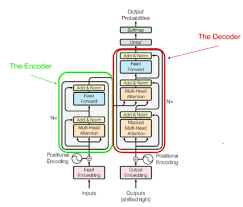
\includegraphics[width=0.45\textwidth]{img/imagesAttention.png}
\caption{The architecture of the proposed summarization model}
\end{figure}

\vspace{1em}
\section*{IV. EXPERIMENTS}
We use a dataset composed of Vietnamese news articles from sources like VnExpress and ZingNews. Evaluation is conducted using ROUGE-1, ROUGE-2, and ROUGE-L metrics.

\begin{table}[H]
\centering
\caption{Evaluation results of the model}
\begin{tabular}{|c|c|c|c|}
\hline
\textbf{Model} & \textbf{ROUGE-1} & \textbf{ROUGE-2} & \textbf{ROUGE-L} \\
\hline
TF-IDF + LSA & 38.2 & 17.3 & 35.0 \\
Proposed Transformer & \textbf{52.5} & \textbf{26.1} & \textbf{48.3} \\
\hline
\end{tabular}
\end{table}

\vspace{1em}
\section*{V. CONCLUSION}
This paper presents a Transformer-based model for Vietnamese text summarization. The model achieves promising results, offering a solid foundation for further research in Vietnamese NLP.

\vspace{1em}
\section*{ACKNOWLEDGMENT}
This research is supported by Vietnam - Korea University of Information and Communication Technology and the VKU AI Research Group.

\vspace{1em}
\section*{REFERENCES}
\begin{enumerate}[label={[{\arabic*}]}]
\item Vaswani et al., ``Attention is All You Need'', NeurIPS, 2017.
\item Raffel et al., ``T5: Exploring the Limits of Transfer Learning'', JMLR, 2020.
\item Nguyen T. H. et al., ``PhoBERT: Pre-trained language models for Vietnamese'', EMNLP, 2020.
\item Lin, C. Y., ``ROUGE: Recall-Oriented Understudy for Gisting Evaluation'', 2004.
\end{enumerate}

\end{document}
